\documentclass[a4paper,10pt]{article}
\usepackage[utf8]{inputenc}
\usepackage[margin=0.7in]{geometry}
\usepackage{amsmath}
\usepackage{algorithm}
\usepackage[noend]{algpseudocode}
\usepackage{tabularx}
\usepackage{graphicx}
\usepackage{amssymb}
\usepackage{enumitem}
\usepackage{comment}
\usepackage{color}
\usepackage[table,xcdraw]{xcolor}
\newlist{todolist}{itemize}{2}
\setlist[todolist]{label=$\square$}
\newcommand{\handout}[5]{
   \renewcommand{\thepage}{}
   \noindent
   \begin{center}
   \framebox{
      \vbox{
    \hbox to 6in { {\bf CSE 141: Introduction to Computer Architecture}
         \hfill #2 }
       \vspace{4mm}
       \hbox to 6in { {\Large \hfill #1  \hfill} }
       \vspace{2mm}
       \hbox to 6in { {\emph{#3} \hfill #4 \emph{#5}} }
      }
   }
   \end{center}
   \vspace*{2mm}
   
   Name: \underline{\hspace{4cm}}
  
   PID: \underline{\hspace{4 cm}}
   
   Email: \underline{\hspace{4 cm}}
}



\newcommand{\homework}[5]{\handout{Final Examination}{#2}{Instructor: #3}{{\bf Due on:} #4}{#5}}

\begin{document}
\homework{1}{Spring 2024}{Jishen Zhao} {June 7, 2024 @ 11:59PM}{(96 points)}

\begin{table}[!hbpt]
    \centering  
    \begin{tabular}{|c|c|c|}
    \hline
    Q1             & 6           &      \hspace{2cm}     \\ \hline
    Q2             & 15           &           \\ \hline
    Q3             & 12           &           \\ \hline
    Q4             & 18          &           \\ \hline
    Q5             & 10          &           \\ \hline
    Q6             & 20          &           \\ \hline
    Q7             & 15          &           \\ \hline
    \textbf{Total} & \textbf{96} & \textbf{} \\ \hline
    \end{tabular}
\end{table}

“While taking this examination, I have not witnessed any wrongdoing, nor have I personally violated any conditions of this course’s integrity policy.” \\ \\ 
If you can honestly attest to the statement above, \textbf{write “I excel with Integrity” below and sign.} \\ \\
If you do not write and sign, the instructor will contact you by e-mail to request you clarify/explain. \\ \\

\noindent\rule{12cm}{0.4pt} \\

\noindent Signature: 

\subsection*{Instructions:}
    \begin{itemize}
    \item This exam is open book and open notes. Show your work and insert your answer in the space(s) provided. Please provide details on how you reach a result unless directed by the question as not to. 
    \item The exam totals 96 points. It counts for 24\% of your course grade. Please submit answers to the following questions as a PDF via Gradescope by June 7, 2024 at 11:59 PM. Policy of late submissions is the same homework assignments. Handwritten or typed responses are accepted.

    \end{itemize}

\subsection*{Reminder:}
\begin{itemize}
\item As a reminder, we will drop the lowest homework grade if class evaluation response rate is above 85\%. This class will adopt the new SET (Student Evaluation of Teaching). You should have received an email with instructions on filling out the evaluation.
\end{itemize}


\pagebreak

\begin{enumerate}
    \item[\textbf{Q1}]{\textbf{(6 points)}: 
        Short answers (no further explanation needed). \\
        \begin{enumerate}
            \item[\textbf{A.}]{Allow cache and memory to be inconsistent, i.e., write the data \textbf{only} into the cache
                block. Is this write-back or write through? \\\rule{3cm}{0.4pt} (No further explanation
                needed)
            }
            \item[\textbf{B.}]{Require cache and memory to be consistent, i.e., always write the data into both
                the cache block and the next level in the memory hierarchy. Is this write-back or
                write through? \\\rule{3cm}{0.4pt} (No further explanation needed)
            }
            \item[\textbf{C.}]{Consider the diagram below that shows the dividing line between the bits used for tag 
                compare and those used to select the cache set. Fill in the lines indicating whether the 
                associativity \textbf{increases} or \textbf{decreases} and whether the resulting cache has only one \textbf{way} or only one \textbf{set}.
                \begin{figure}[!hbpt]
                    \centerline{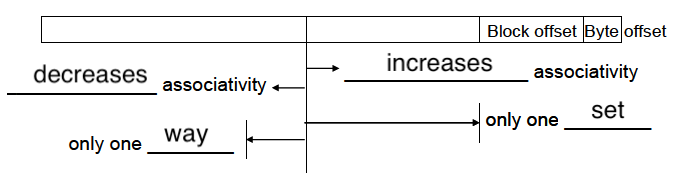
\includegraphics[scale = 0.7]{cacheAssociativity.png}}
                    \label{cacheAssociativity}
                \end{figure}
            }
        \end{enumerate}
    }
    \item[\textbf{Q2}]{\textbf{(15 points)}: Cache Performance \\
    
        Assuming the base $CPI_{base}$ (no stall) of a pipeline is 1. A program has 25\% of load/store 
        instructions. The processor only has one level of cache, i.e., an L1 instruction cache and 
        an L1 data cache. Cache miss rate and penalty are as following:
        
         \begin{itemize}
            \item{L1 instruction cache : $\%_{miss}$ = 2\%, $t_{miss} = 30$ cycles}
            \item{L1 data cache: $\%_{miss}$ = 30\%, $t_{miss} = 30$ cycles}
         \end{itemize}
         
        What is the CPI?
        %\vspace{4cm}
        \pagebreak
    }
    
    \item[\textbf{Q3}]{\textbf{(12 points):} Cache tag overhead \\
    
        Assume:
        \begin{itemize}
            \item A processor has a 64KB 4-way set associative cache
            \item The cache access uses physical addresses only
            \item A physical address is 48 bits long 
            \item Each block holds 64 bytes of data
            \item Tag overhead includes the valid bit and tag bits
        \end{itemize}
        
        How much is the tag overhead in percent (no need to consider dirty bit)?
        \pagebreak
    }
    \item[\textbf{Q4}]{\textbf{(18 points):} Multicore: Cache Coherence \\ 
    
        Assuming write-back caches, private L1 data caches (L1Ds) (no L2), shared memory, 
        and a MESI coherence policy, indicate in the cache tables what would 
        be the values (V) of the variables X and Y and their coherency (C) state (either M, E, S or
        I) in the L1D’s for a dual core processor with the following sequence of reads and writes. 
        As shown in the table, the coherency (C) state in Step 0 (the initial coherency state) of 
        both variables in both caches is I (invalid). If a value doesn’t change, you may leave that 
        entry blank. You may use either the state transition diagram or the table given below to 
        reason about cache coherence.
        
        \begin{itemize}
            \item[Step 0: ]{Initially, X =3, Y = 5 in the shared memory, processor caches are empty}
            \item[Step 1: ]{Core 1 reads X (from the shared memory)}
            \item[Step 2: ]{Core 2 reads X}
            \item[Step 3: ]{Core 1 writes X = 2}
            \item[Step 4: ]{Core 1 writes Y = 6}
            \item[Step 5: ]{Core 2 reads Y}
        \end{itemize}
        
        Please fill in the following cache and shared memory tables (no further explanation for your answers is required).
        
        % Please add the following required packages to your document preamble:
        % \usepackage[table,xcdraw]{xcolor}
        % If you use beamer only pass "xcolor=table" option, i.e. \documentclass[xcolor=table]{beamer}
        \begin{table}[!hbpt]
        \centering
        \begin{tabular}{|ccccccccccccc|}
        \hline
        \multicolumn{13}{|c|}{Core 1's L1D Cache (private)}                                                                                                                                                                                                                                                                                                                                                                                                             \\ \hline
        \multicolumn{1}{|c|}{}  & \multicolumn{2}{c|}{Step 0}                      & \multicolumn{2}{c|}{\cellcolor[HTML]{C0C0C0}Step 1}                                             & \multicolumn{2}{c|}{Step 2}                     & \multicolumn{2}{c|}{\cellcolor[HTML]{C0C0C0}Step 3}                                             & \multicolumn{2}{c|}{Step 4}                     & \multicolumn{2}{c|}{\cellcolor[HTML]{C0C0C0}Step 5}                        \\ \hline
        \multicolumn{1}{|c|}{}  & \multicolumn{1}{c|}{V}  & \multicolumn{1}{c|}{C} & \multicolumn{1}{c|}{\cellcolor[HTML]{C0C0C0}V} & \multicolumn{1}{c|}{\cellcolor[HTML]{C0C0C0}C} & \multicolumn{1}{c|}{V} & \multicolumn{1}{c|}{C} & \multicolumn{1}{c|}{\cellcolor[HTML]{C0C0C0}V} & \multicolumn{1}{c|}{\cellcolor[HTML]{C0C0C0}C} & \multicolumn{1}{c|}{V} & \multicolumn{1}{c|}{C} & \multicolumn{1}{c|}{\cellcolor[HTML]{C0C0C0}V} & \cellcolor[HTML]{C0C0C0}C \\ \hline
        \multicolumn{1}{|c|}{X} & \multicolumn{1}{c|}{--} & \multicolumn{1}{c|}{I} & \multicolumn{1}{c|}{\cellcolor[HTML]{C0C0C0}}  & \multicolumn{1}{c|}{\cellcolor[HTML]{C0C0C0}}  & \multicolumn{1}{c|}{}  & \multicolumn{1}{c|}{}  & \multicolumn{1}{c|}{\cellcolor[HTML]{C0C0C0}}  & \multicolumn{1}{c|}{\cellcolor[HTML]{C0C0C0}}  & \multicolumn{1}{c|}{}  & \multicolumn{1}{c|}{}  & \multicolumn{1}{c|}{\cellcolor[HTML]{C0C0C0}}  & \cellcolor[HTML]{C0C0C0}  \\ \hline
        \multicolumn{1}{|c|}{Y} & \multicolumn{1}{c|}{--} & \multicolumn{1}{c|}{I} & \multicolumn{1}{c|}{\cellcolor[HTML]{C0C0C0}}  & \multicolumn{1}{c|}{\cellcolor[HTML]{C0C0C0}}  & \multicolumn{1}{c|}{}  & \multicolumn{1}{c|}{}  & \multicolumn{1}{c|}{\cellcolor[HTML]{C0C0C0}}  & \multicolumn{1}{c|}{\cellcolor[HTML]{C0C0C0}}  & \multicolumn{1}{c|}{}  & \multicolumn{1}{c|}{}  & \multicolumn{1}{c|}{\cellcolor[HTML]{C0C0C0}}  & \cellcolor[HTML]{C0C0C0}  \\ \hline
        \end{tabular}
        \end{table}
        
        \begin{table}[!hbpt]
        \centering
        \begin{tabular}{|ccccccccccccc|}
        \hline
        \multicolumn{13}{|c|}{Core 2's L1D Cache (private)}                                                                                                                                                                                                                                                                                                                                                                                                             \\ \hline
        \multicolumn{1}{|c|}{}  & \multicolumn{2}{c|}{Step 0}                      & \multicolumn{2}{c|}{\cellcolor[HTML]{C0C0C0}Step 1}                                             & \multicolumn{2}{c|}{Step 2}                     & \multicolumn{2}{c|}{\cellcolor[HTML]{C0C0C0}Step 3}                                             & \multicolumn{2}{c|}{Step 4}                     & \multicolumn{2}{c|}{\cellcolor[HTML]{C0C0C0}Step 5}                        \\ \hline
        \multicolumn{1}{|c|}{}  & \multicolumn{1}{c|}{V}  & \multicolumn{1}{c|}{C} & \multicolumn{1}{c|}{\cellcolor[HTML]{C0C0C0}V} & \multicolumn{1}{c|}{\cellcolor[HTML]{C0C0C0}C} & \multicolumn{1}{c|}{V} & \multicolumn{1}{c|}{C} & \multicolumn{1}{c|}{\cellcolor[HTML]{C0C0C0}V} & \multicolumn{1}{c|}{\cellcolor[HTML]{C0C0C0}C} & \multicolumn{1}{c|}{V} & \multicolumn{1}{c|}{C} & \multicolumn{1}{c|}{\cellcolor[HTML]{C0C0C0}V} & \cellcolor[HTML]{C0C0C0}C \\ \hline
        \multicolumn{1}{|c|}{X} & \multicolumn{1}{c|}{--} & \multicolumn{1}{c|}{I} & \multicolumn{1}{c|}{\cellcolor[HTML]{C0C0C0}}  & \multicolumn{1}{c|}{\cellcolor[HTML]{C0C0C0}}  & \multicolumn{1}{c|}{}  & \multicolumn{1}{c|}{}  & \multicolumn{1}{c|}{\cellcolor[HTML]{C0C0C0}}  & \multicolumn{1}{c|}{\cellcolor[HTML]{C0C0C0}}  & \multicolumn{1}{c|}{}  & \multicolumn{1}{c|}{}  & \multicolumn{1}{c|}{\cellcolor[HTML]{C0C0C0}}  & \cellcolor[HTML]{C0C0C0}  \\ \hline
        \multicolumn{1}{|c|}{Y} & \multicolumn{1}{c|}{--} & \multicolumn{1}{c|}{I} & \multicolumn{1}{c|}{\cellcolor[HTML]{C0C0C0}}  & \multicolumn{1}{c|}{\cellcolor[HTML]{C0C0C0}}  & \multicolumn{1}{c|}{}  & \multicolumn{1}{c|}{}  & \multicolumn{1}{c|}{\cellcolor[HTML]{C0C0C0}}  & \multicolumn{1}{c|}{\cellcolor[HTML]{C0C0C0}}  & \multicolumn{1}{c|}{}  & \multicolumn{1}{c|}{}  & \multicolumn{1}{c|}{\cellcolor[HTML]{C0C0C0}}  & \cellcolor[HTML]{C0C0C0}  \\ \hline
        \end{tabular}
        \end{table}
        
        \begin{table}[!hbpt]
        \centering
        \begin{tabular}{|ccccccc|}
        \hline
        \multicolumn{7}{|c|}{Shared memory}                                                                                                                                                                                                                            \\ \hline
        \multicolumn{1}{|c|}{}  & \multicolumn{1}{c|}{Step 0} & \multicolumn{1}{c|}{\cellcolor[HTML]{C0C0C0}Step 1} & \multicolumn{1}{c|}{Step 2} & \multicolumn{1}{c|}{\cellcolor[HTML]{C0C0C0}Step 3} & \multicolumn{1}{c|}{Step 4} & \cellcolor[HTML]{C0C0C0}Step 5 \\ \hline
        \multicolumn{1}{|c|}{}  & \multicolumn{1}{c|}{V}      & \multicolumn{1}{c|}{\cellcolor[HTML]{C0C0C0}V}      & \multicolumn{1}{c|}{V}      & \multicolumn{1}{c|}{\cellcolor[HTML]{C0C0C0}V}      & \multicolumn{1}{c|}{V}      & \cellcolor[HTML]{C0C0C0}V      \\ \hline
        \multicolumn{1}{|c|}{X} & \multicolumn{1}{c|}{3}      & \multicolumn{1}{c|}{\cellcolor[HTML]{C0C0C0}}       & \multicolumn{1}{c|}{}       & \multicolumn{1}{c|}{\cellcolor[HTML]{C0C0C0}}       & \multicolumn{1}{c|}{}       & \cellcolor[HTML]{C0C0C0}       \\ \hline
        \multicolumn{1}{|c|}{Y} & \multicolumn{1}{c|}{5}      & \multicolumn{1}{c|}{\cellcolor[HTML]{C0C0C0}}       & \multicolumn{1}{c|}{}       & \multicolumn{1}{c|}{\cellcolor[HTML]{C0C0C0}}       & \multicolumn{1}{c|}{}       & \cellcolor[HTML]{C0C0C0}       \\ \hline
        \end{tabular}
        \end{table}
        
        \pagebreak
    }
    \item[\textbf{Q5}]{\textbf{(10 points):} Memory consistency \\ 
    
        Two threads (A and B) are concurrently running on a dual-core processor that 
        implements a sequentially consistent memory model. Assume that the value at address 
        (R10) is initialized to 0. The instruction \texttt{st immediate, (R10)} writes an immediate 
        number into the memory address stored in R10.
        
        \begin{table}[!hbpt]
        \centering
        \begin{tabular}{|cccc|}
        \hline
        \multicolumn{4}{|c|}{\textbf{Thread A (core 1)}} \\
        1:        & st        & 0x1,       & (R10)       \\
        2:        & ld        & R1,        & (R10)       \\
        3:        & st        & 0x2,       & (R10)       \\
        4:        & ld        & R2,        & (R10)       \\ \hline
        \end{tabular}
        \quad
        \quad
        \begin{tabular}{|cccc|}
        \hline
        \multicolumn{4}{|c|}{\textbf{Thread B (core 2)}} \\
        1:        & st        & 0x3,       & (R10)       \\
        2:        & ld        & R3,        & (R10)       \\
        3:        & st        & 0x4,       & (R10)       \\
        4:        & ld        & R4,        & (R10)       \\ \hline
        \end{tabular}
        \end{table}
        
        After both threads have finished executing, you find that (R1, R2, R3, R4) = (1, 2, 3, 4). 
How many different instruction orderings of the two threads produce this result (please show all possible orderings)?
        \pagebreak
    }
    \item[\textbf{Q6}]{\textbf{(20 points):} Main Memory
    
    Given a system with 2 memory channels and 4 DRAM DIMMs (2 DIMMs per channel), each DIMM has:
        
    \begin{itemize}
        \item 1 rank per DIMM
        \item 8 chips per rank
        \item 8 bits per column
        \item 8 banks per chip
        \item 32,768 rows per bank
        \item 2,048 columns per bank
    \end{itemize}


    \begin{enumerate}
        \item[A)]{What is the total amount (bytes) of physical memory in the system?
        \vspace{5cm}}
        \item[B)]{What is the minimum number of physical address bits needed to address this much
memory?\vspace{5cm}}
        \item[C)]{With the number of physical address bits obtained in B), also assume
            \begin{itemize}
                \item The physical address space has 1M (i.e., 1048576) pages (physical frames)
                \item Virtual addresses have 64 bits
            \end{itemize}
            What is the maximum number of pages in the virtual address space?
        }
    \end{enumerate}
    \pagebreak
    }
    \item[\textbf{Q7}]{\textbf{(15 points):} GPUs
    
    \begin{enumerate}
        \item[A)]{
        Which ones of the following are the basic ideas of GPU processor architecture design? (Multiple selections, no further explanation needed.)
            \begin{todolist}
                \item Interleave processing of many fragments on a single core to avoid stalls caused by high latency operations
                \item Make common case fast
                \item Remove components that help a single instruction stream fast
                \item Amortize cost/complexity of managing an instruction across many ALUs
            \end{todolist}
        }
        \item[B)]{
            Assume a hypothetical GPU with the following characteristics:
            
            \begin{itemize}
                \item Clock rate 1 GHz
                \item 32 simultaneous instruction streams
                \item Contains 8 SIMD cores, each containing 32 single-precision floating-point units, each instruction performs one single-precision floating-point operation (either a multiply or an add)
                \item 1024 concurrent (but interleaved) instruction streams
            \end{itemize}
            
            What is the peak single-precision floating-point throughput for this GPU in GFLOP/sec, assuming that all memory latencies can be hidden? 
        }
    \end{enumerate}
    
    }
    
\end{enumerate}


\end{document}


% (1,2) (3, 4) (5, 7) (6)